\documentclass[a4paper, twoside, 11pt]{report}
%pridat documentclass[twoside] - pro tisk
%\input{thesis_settings/page_settings}
\usepackage{xcolor}
\usepackage[colorinlistoftodos, textsize=tiny]{todonotes}
\usepackage[top=2cm,bottom=2cm, left=3cm, right=2cm]{geometry}
\usepackage{graphicx}
\usepackage{wrapfig}
\usepackage[utf8]{inputenc}
\usepackage[linktoc=all]{hyperref}
%\usepackage[czech]{babel}
\usepackage[utf8]{inputenc}
\usepackage[T1]{fontenc}
\usepackage{needspace}
%\usepackage{fontspec}
\usepackage{calc}
\graphicspath{ {images/} }
%
\newcommand\pro{\item[$+$]}
\newcommand\con{\item[$-$]}
%
\begin{document}
%
\begin{titlepage}
\title{Introduction to\\Additive Manufacturing Technologies}
\author{Martin Hejtmanek}
\date{28.2.2017}
\maketitle
\end{titlepage}
%
\chapter*{Acknowledgements}
Esa kontio, Jiři Moravec, Pruša, Tata

\chapter*{List of shortcuts}
\addcontentsline{toc}{chapter}{List of shortcuts}
\begin{itemize}
\item[AM]Additive manufacturing
\item[BJ]Binder jetting
\item[DED]Directed energy deposition
\item[DMD]Digital micromirror device
\item[DMLS]Direct metal laser sintering
\item[EBM]Electron beam melting
\item[FDM]Fused deposition modeling
\item[FFF]Fused filament fabrication
\item[LOM]Laminated object manufacturing
\item[MJ]Material jetting
\item[PBF]Powder bed fusion
\item[SL]Sheet lamination
\item[SLA]Stereolitography
\item[SLS]Selective laser sintering
\item[STL]Stereolitography or STL file format
\end{itemize}


\chapter{Introduction}
%
%
%
\section{About the thesis}
There are many terms like Additive Manufacturing, 3D printing, rapid prototyping and more, that are used to describe specific technologies. Although they are not precisely synonyms, all of them are related to a specific way of product manufacturing. Nowadays, we are still used to making machines and parts from solid blocks of raw material, and then machining away material until desired shape if acquired. Also casting, forming, welding and other technologies are used in the classical process chain, in order to make a specific part.\\
However, since 1980s there were new and different manufacturing technologies being developed, that used vastly different approach. This trend still continues with more and more interest being paid to this field. Those technologies are commonly named \textbf{Additive manufacturing technologies} (hereinafter AM). The main underlying principle of all AM technologies, that will be listed later, is making part by adding material, instead of removing it. This approach has many advantages over previously mentioned conventional technologies, but it also brings different problem sets that need to be solved.\\
As mentioned, AM technologies are on a rise. It is now more than 30 years since humble beginnings of the first AM technology, Stereolitography. Since then, AM industry developed rapidly and is today worth several billions of dollars on the market. Its significance can"t be stressed out enough, and sometimes we are not paying as much attention to AM as we should. It takes a lot of time to fully realize, how big difference in terms of parts production AM can cause. Sometimes we might not realize, that parts we are used to make using classical approach, could be made using AM, faster and without perfectly planned pre-production planning, post-production and with less waste material. AM technologies were not developed to replace conventional technologies - they will probably always have its place on the market. Still, conventional processes can be supported by AM when possible in order to increase manufacturing speed, simplicity and reduce product price. There are even available machines, trying to merge CNCs and AM into a single functional production machine.\\
For the problematic of AM machines is very complex, choosing a single technology and fully describing it into detail would be sufficient for diploma thesis. Therefore it is out of scope of this BT, to give detailed description of all technologies. There are many intricate processes included, related to heat and mass transfer, material processing and properties, precise positioning systems, careful regulation of build environment conditions and much more.\\
\textbf{The main goal of this Bachelor thesis} is to make research on the AM field and available technologies. Then, make a brief, but complete and understandable summary of them and describe ongoing processes. This BT should give the reader an opportunity to understand essentials of individual technologies - know their strengths, weaknesses, main working principles and for which applications are they suitable.\\
The future of AM market is still to unfold, but statistics are showing that AM machines will be used more in production process - especially with the continuous trend of improving materials availability, development of new materials or price reduction of all key electronic / mechanical parts. \newpage
%
\section{Resources}
In this thesis, I use primarily limited amount of resources and literature. Even though this thesis should be complex and diverse, I decided to use the book \cite{AMT} as my primary source of information. This book is than supplemented by facts from scientific journals, other books, information from AM machine vendors, webpages and others. Also, there are sections where I write information gained at OAMK (mentioned in the acknowledgement), so the information source can't be easily told.\\
The reason for using \cite{AMT} as my primary information source is simple - this book is very up-to date, and goes deep into the topics well enough. This more than 500 pages book is professional well enough . It covers all the details of almost any AM-related problematic, and full understanding the complete content requires high level of education in chemistry, calculus, material engineering and more. Since it is out of my scope, even to fully understand this book itself, I believe taking it as a primary information source is acceptable, and will not cause the thesis to be too simple due to lack of resources.
%
\section{Additive manufacturing and process engineering}
Since this thesis is made under the auspices of Department of Process Engineering, it should be mentioned why AM is relevant to this engineering field. At the first glance, we might think that since AM is a production technology, it should be inspected and researched mostly be material and technology engineers. However, as it will be mentioned, AM is incredibly intricate and wide field, which requires understanding of many ongoing processes, because almost everything during AM process is related together. Even though not directly, one parameter of the machine may easily affect other parameters, which in turn have impact on the final part properties and build success. These processes very often involve heat transfer, mass transfer, controlling conditions of the build environment, flow of viscous fluids, chemical curing and others. All of these processes should be generally understood by process engineers. Such processes are usually dealt with in fields like food industry, pharmaceutic, distilleries, breweries, water cleaning, oil refinery and many others. However, physics apply here same as anywhere and the equations are applicable for AM processes all the same.\\
Following is a table of application of processes solved by process engineers, applied on field of AM.
\\[10pt]
\begin{tabular}{||c||c||c|}
\hline 
\textit{Problematic} & \textit{Common application} & \textit{AM application} \\ 
\hline 
\textbf{Heat transfer} & Heat exchangers balance & PBF build heating and cooling \\
\hline
\textbf{Mass transfer} & Filters for particle separation & SLS sintering, particle fusion \\ 
\hline 
\textbf{Inert atmosphere} & Food packaging & Preventing oxidation with PBF or DED\\
\hline 
\textbf{Droplet formation} & Cooling by evaporation & Material jetting nozzle droplet \\ 
\hline 
\textbf{Viscous fluid flow} & Food industry, dough flow & FDM nozzle flow, Material jetting nozzles\\ 
\hline 
\textbf{Chemical reactions} & Bio reactors & SLA curing\\ 
\hline 
\end{tabular} 
%
\section{Terminology}
This thesis has the term AM in its name. That doesn't mean other terms couldn't have been used instead. I will mention similar terms commonly used in context of production technologies.\\
From all mentioned possibilities, I choose to use term \textbf{"Additive manufacturing"} – AM in this thesis, because it is the most commonly used one. In Czech language, term "3D printing" could have been used. The reason is that people are familiar with home 2D printers, hence the term is easy to use and remember. There is no point in saying that one term is better to use than the other one – it is matter of choice. For me, the term AM fits the purpose of this BT the most.

\subsection{Automated fabrication}
Term \textbf{"Automated fabrication"} was used before AM. It was supposed to emphasize the fact that computers and controllers could take control of manufacturing processes, making them more efficient and easier to perform.
\subsection{Freedom fabrication}
\textbf{"Freedom Fabrication"} term was used to imply that the build time of a part doesn't depend on the geometry. In other words, the rule "the more complex parts, the longer time to build it takes", which is usually applied with conventional production methods, doesn't apply here.
\subsection{Additive Manufacturing}
\textbf{"Additive manufacturing"} term is saying that we are adding material to build the part instead of removing it.
\subsection{3D printing}
\textbf{"3D printing"} term was mainly used within MIT researchers, and was implying the application of common 2D printers and adding a third dimension.
\subsection{Rapid prototyping}
\textbf{"Rapid prototyping"} was term used in connection with additive manufacturing. It is telling us nothing about any specific technologies. Instead, it is emphasizing the speed and ease of AM compared to conventional prototyping methods. Rapid prototyping is saying that with AM, one is able to make functional prototypes faster and cheaper, all of that without any other special equipment needed.\\
\\
\cite[p.~7]{AMT}
%
%
%
\chapter{About AM in general}
%
\section{History of AM}
First of all, it is important to note that development of AM technologies can't be separated from development in related fields. We can say that \textbf{AM machines consist of many intricate sub-systems}. For example, very precise and fast positioning system are required. Powerful lasers are used to melt and fuse material together. Computers, micro controllers and electronics in general are required to control the environment and guide the build process. Last but not least, materials were developed to suit specific AM technology. Without these and many more improvements, there would be no machines like the ones today. When we compare nowadays machines and the ones from AM beginnings, first machines would be slower and less precise, would encountered material behavior problems, would be more buggy, but most importantly – much more costly.\\
AM has been out there longer than it might appear. It is not technology of 21st century, but it originates in 1970s / 1980s. Back then, there were only conventional methods, but for the first time, attention was paid to possibility of curing photopolymers into specific shape in. An idea was developed to make use of additive production using layer approach – construction of separate layers, merging into final product.\cite{AMOrigins}\\
%
\begin{wrapfigure}{r}{0.5\textwidth}
 	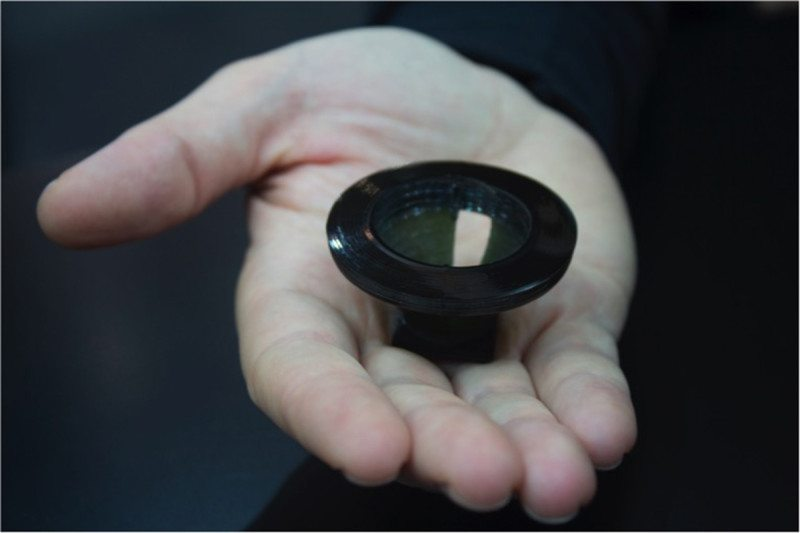
\includegraphics[width=\textwidth/2]{firstPrintedObject}
	\caption{First object made with AM}
\end{wrapfigure}
%
\\
The first commercialized AM technology was \textbf{Stereolitography} (STL). There were experiments with curing layers of photopolymer resins simultaneously, thus creating separate layers. It was in Japan in 1981, when first schematics of possible technology using photopolymer-hardening were described and proven to work. Later in 1984-1986, Charles Hull filed the patent for the first working machine.\cite{FirstPatent}
In 1986, he also founded “3D systems” company, which was probably the first company to do business with 3D printers. Nevertheless, Charles Hull is also important for his contribution to AM field by work on the “STL file format” – a specific format used by computers for describing the geometry of fabricated parts. (Will be described later).\\
Technology that emerged later was \textbf{“Fused deposition modeling”} (FDM). This technology is using plastic material in a form of wire, which is molten and deposited into a single layer. The patent for FDM was filed in 1989 by S. Scott Crump from Stratasys Inc.  - also very important company in AM business that is still in operation.\\
In the first half of 90s, remaining technologies were starting to be commercialized. They usually went under their specific names like "Selective laser sintering" or  "Laminated object manufacturing". These technologies were filling in gaps in missing technologies of "Powder bed fusion" (PBF), "Sheet Lamination" (SL), "Material jetting" (MJ) and "Binder jetting" (BJ) ; there is no need for naming all individual patents.\\
When we mention patents and copyrights, we have to realize that patents have a major impact on development of AM. Technologies, processes and even materials from AM are subjected to patents. When patents are no longer held after 25 years, the competitiveness of other companies grows, resulting in bigger supply of AM machines and their price reduction. Expiration of patents was one of the reasons, why we experienced rapid growth of FDM machines.

\section{Comparison of AM and CNC machining}
%
Before I describe and categorize basic AM processes, it is important to see the \textbf{distinction between AM and conventional CNC manufacturing}. The reason being, both approach the same problem of manufacturing from different point of view.\\
Conventional manufacturing processes are based on machining and processing block of raw material, thus it is \textit{subtractive process}. Using modern equipment, one is able to achieve very high precision of manufactured part with good surface quality. Materials such as steel and other metals are commonly utilized, alongside with plastics, wood and many other materials that can be processed. However, in general often parts of complex shapes could be very tricky to make. With CNCs, it is impossible to create objects with inner cavities or other internal features by machining the inside of the object. Also, machining shapes like curved overhangs or crevasses can be problematic. Furthermore, we haven’t considered the amount of waste material yet. Because we need block of raw material, exceeding the dimensions of the part made in all directions, it is not rare to machine away more than 80\% of material. This material then becomes waste material. Although scrap material is recycled, the blocks of raw material can be very expensive. Machining parts for use in aerospace industry might be a typical example. The parts are often of very complex shape, and made out of lightweight metals such as titanium. Requiring big block of titanium can be unnecessarily expensive - significant part of provided material in fact is unused and thrown away.\\
Another field of comparison of AM and conventional production processes is the scale and amount of produced parts. Conventional methods of machining are known for a long time, and are used for series production. The combination of CNC machining with i.e. mold casting is a fast and efficient process. Regarding these series-process chains, problems will occur when we want to alter a few manufactured parts. It is not suitable for making only few parts because of long preparation time, prototyping phase, and expensive equipment needed specially only for one kind of a product.\\
As it follows from the name itself, AM is not subtractive, but \textit{additive manufacturing process}. Most of AM technologies are not limited by mentioned obstacles of CNC, such as manufacturing inner cavities or producing waste material. The simple idea, depositing material only where we want, results in having almost no waste material. Some technologies require material recycling though, but recycled material is immediately ready for use. Because AM machines are based on material deposition instead of removal, time of product manufacturing is almost \textbf{independent of it's shape}. In other words, AM machines don't care if we print a box, statue or a scaled model of a flower. The build time depends only on the amount of material deposited.\\
This attribute comes very handy in production of single custom parts of complicated shapes. The example might be printing custom body-parts of implants, since they are always unique, person to person. Also, shape-free manufacturing comes very handy to designers, who used to encounter limitations of capabilities of conventional machines, making production of complex shapes tricky.\\
For the comparison to be complete, it should also be mentioned that machining is often not suitable for processing hard and brittle materials. On the other hand, machining results in almost "isotropic part", if the material itself is isotropic. Meaning, there shouldn't be differences in machined part related to the direction of CNC tool movement. With AM, this is never the case - there is always some some amount of unisotrophy, caused by building the part in different manner in Z-direction compared to X-Y directions.\\
When we look at AM processes, we see a major difference - waste material is no longer a problem. When we want to produce small number of customized parts or objects, AM enables us to do so. The general process of object making (of course depending on specific technology) takes longer time, but considered that i.e. complex parts can be manufactured simultaneously in one go, they don't have to be moved from machine to machine. This may cause significant time savings, resulting in faster production process, even though the technology itself is not faster than CNC. Of course different technologies differ in build-speed.
\begin{figure}[h]
\centering
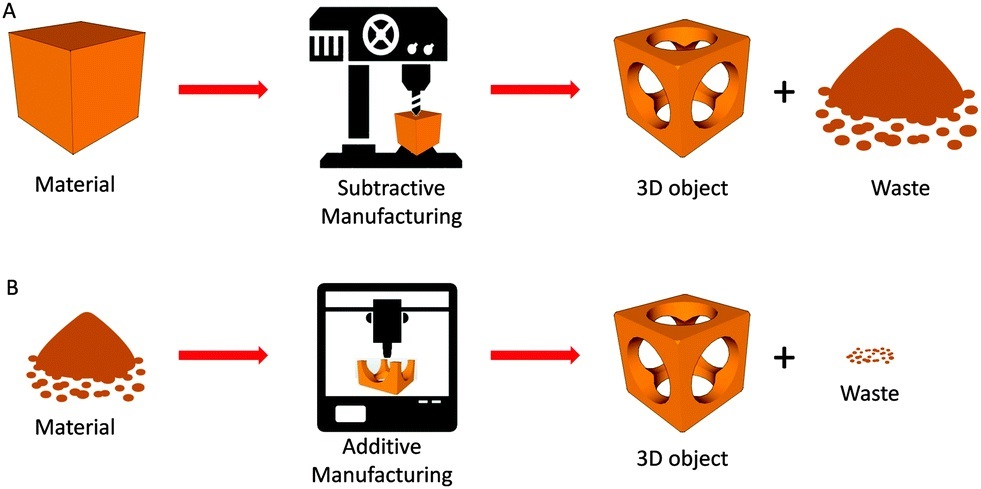
\includegraphics[scale=0.6]{additiveSubtractiveManufacturing}
\caption{Additive vs subtractive manufacturing illustration}
\end{figure}

\section{What precedes part production - AM process chain}
If we want to make use of modern AM machines, we have to be able to prepare everything necessary. Same as with other manufacturing  technologies, making parts using AM \textbf{requires} more or less \textbf{preparation}, and sometimes also \textbf{post-processing} is required. Let's look at the necessary steps, preceding or following the part making.\\
\subsection{Information about produced part}
If we take it from the very beginning, we have to start with knowledge of part to be produced. We have to know what are we building. This information is actually virtual model of a part. Virtual model in electronic form can be handled by computer and converted to other formats, which AM machines accept. There are more ways of creating virtual model of the part, but probably only two methods are used.
\subsubsection{CAD modeling}
When possible, it is obvious that creating model using CAD software can be the most efficient solution. When we use modern CAD systems, changing virtual model doesn't require much effort. It is very useful, if we are planning to make some changes with produced part - we are iterating and changing every version to make the part better. With CAD, it can be matter of a few minutes / hours to make new model and print it. With mass production tools, this process of iterations and changes of production tools (such as casting tools) can be very time and money-consuming.
\subsubsection{AM and reverse engineering}
It can also happen that we want to produce part, but we can't make use of CAD software. The part can be too complicated to create a model, and modeling would be inefficient. If we already have a part we want to build, i.e. we want to "copy" a real existing part, we can make a virtual model using some 3D scanning system or device. There are many devices on the market, enabling us to do so. Scanning devices vary in properties. Easiest criteria for their classification is to distinguish between \textbf{contact and non-contact scanning devices}. Examples of contact scanning device can be machines used in metrology for precise part measurement. Precision of several micrometers can be achieved.\\
%
\begin{figure}[h]
  \centering
  \begin{minipage}[t]{0.4\textwidth}
    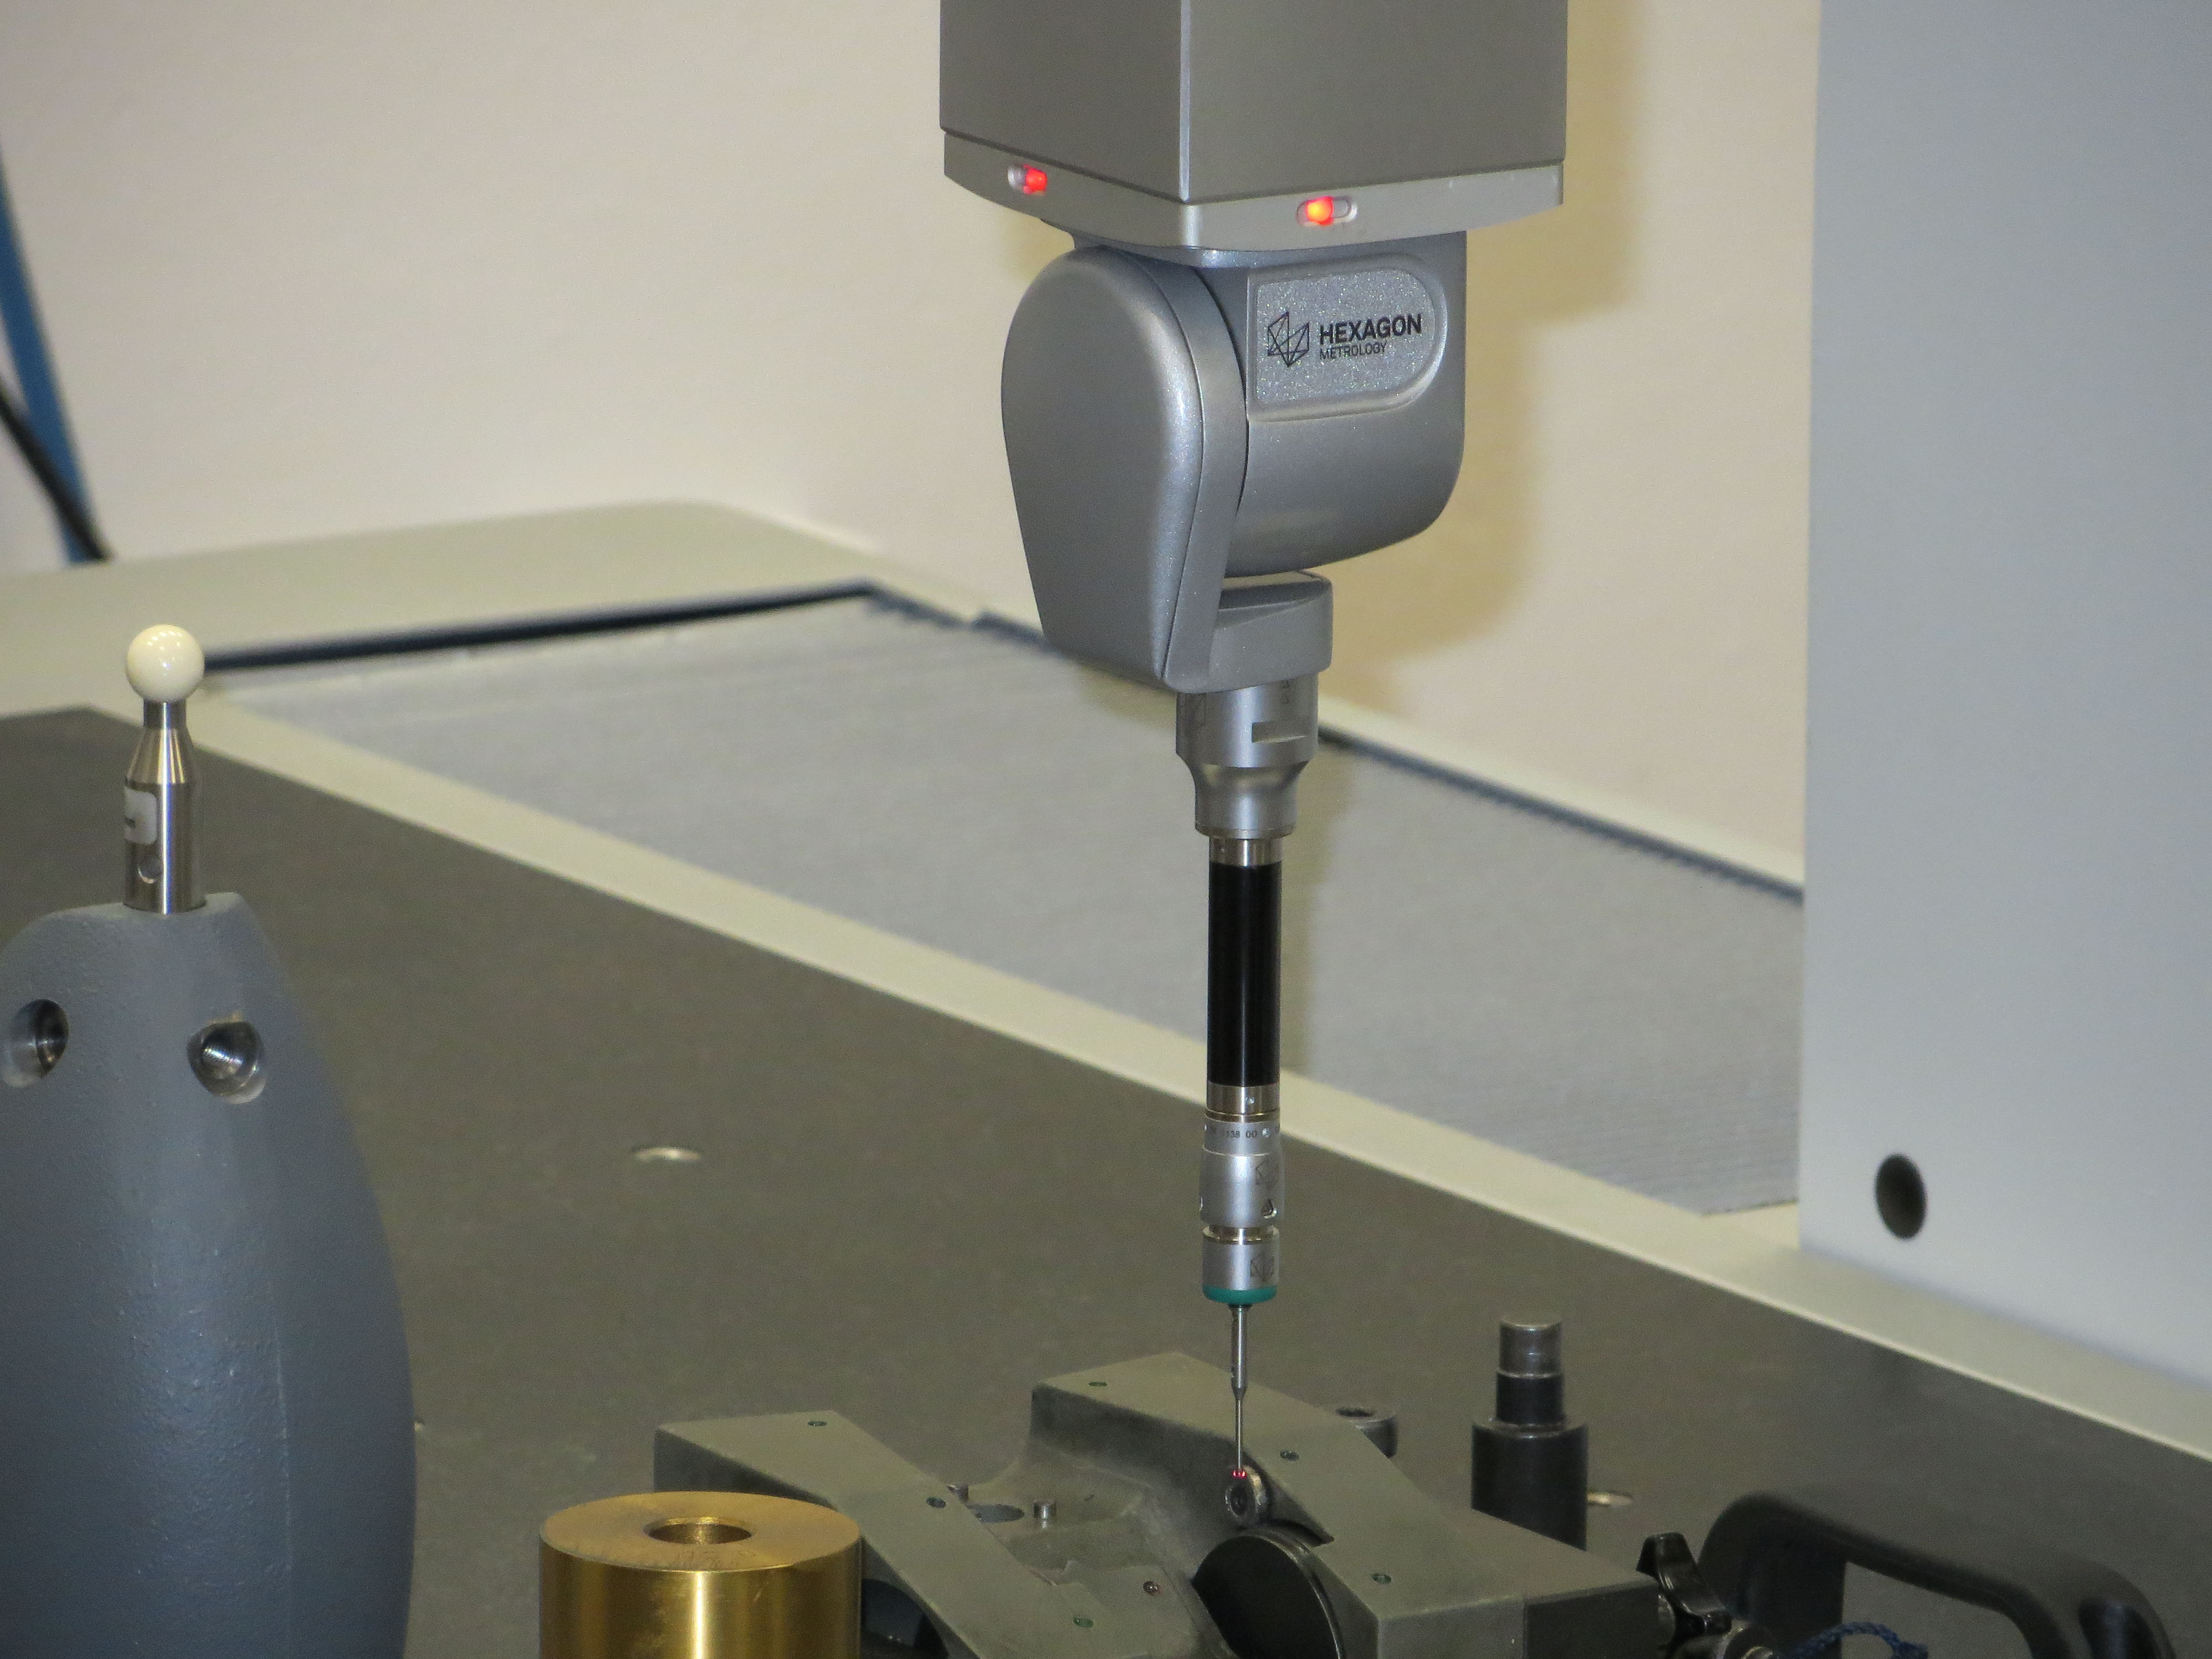
\includegraphics[width=\textwidth]{scanningMachine1}
  \end{minipage}
  \hfill
  \begin{minipage}[t]{0.4\textwidth}
    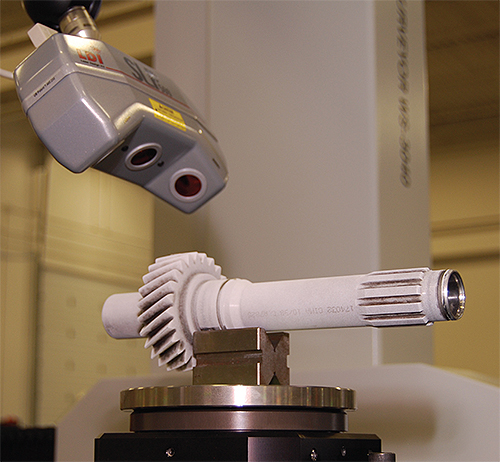
\includegraphics[width=\textwidth]{scanningMachine2}
  \end{minipage}
  \\[5pt]
  \begin{minipage}[b]{0.4\textwidth}
    \caption{Coordinate measuring machine}
  \end{minipage}
  \hfill
  \begin{minipage}[b]{0.4\textwidth}
    \caption{Non-contact laser scanning system}
  \end{minipage}
\end{figure}
%



    
Non-contact scanning devices vary in methods of measuring. Lasers can be utilized for distance measuring, or optical systems can be used. It is even possible with special photographic / optical software to obtain 3D model from multiple pictures of an object. Also, methods already utilized in medical field can be used - MRI machines or CT machines (micro-CT respectively) have been in use for several decades for medical purposes. Today, we can extend the use of these technologies, and use them as very precise scanning devices.
\subsubsection{File formats for AM software}
After obtaining the data, PC processing follows. Software for use with AM machines usually accept only specific data formats. The most common, that was already mentioned, is the \textbf{"STL" file format}.\\
Although it is not essential to know, how the file format represents the geometry of the part, it can be useful to know, because it is possible that some glitches or errors can happen during processing. If we know the format specifics, we can guess where the problem can be. When it comes to "STL" file format, it represents the whole geometry with triangles - it creates a mesh of points on the whole surface of the part, and then connects the nodes to form triangles. That means if we want to accurately represent part geometry, with stl we have to have very fine mesh of points - The greater the distances between mesh nodes are, the bigger imperfections of the virtual model will be.\\
STL file format is generally still accepted by AM machines, but it has some drawbacks. The biggest one is, the part geometry is the only thing it can describe. With modern AM machines, that is not enough, if we want to include additional information about the part in a single file. That is where additive manufacturing format -\textbf{"AMF" file format} comes in. AMF format enables us to describe, among other attributes, color of part for multi-color machines, material specification, or lattices and constellations within the part.
\subsection{Further data manipulation}
As expected, the AM machine itself doesn't accept nor "AMF" or "STL" file format. Since AM machine builds the part layer by layer, it only needs to know how to build each separate layer. Therefore we have to use software called \textbf{Slicer}. Each AM machine will have it's specification, but generally speaking, the output of the slicer should be a file with information, representing 2D shape of each layer. The machine itself then deals with the build process itself and starts printing layers - it doesn't care about their shape, it only deals with mechanics and kinematics of the building system.
\subsection{Machine preparation}
When the data are processed and ready to be sent to the machine, last remaining thing to be done before the build is the machine preparation. In some cases, there might be no need for any further preparation. With machines utilizing some kind of heat processing of material, preheating is often done. With PBF for example, preheating of the build space to high temperatures is done. Same with FDM machines, the metal extrusion nozzle is always heated to build temperature. Apart from preheating, some additional actions can be made, such as often crucial machine calibration or checking for any errors before build starts. Preparation stage is very important and shouldn't be neglected - small imperfection in the built part, caused by wrong machine preparation, can easily cause problems during the build process and ruin final product.
\subsection{Post-processing}
When we remove the built part, it might need some additional care to be ready for use. If building process heated the part, we usually wait until the part cools to ambient temperature to be processed further. Part removal is not always simple. With PBF technology, the excessive powder has to removed and the part cleaned, usually by blowing pressurized air. Same with Stereolitography or Binder jetting, we have to clean the part from excessive photopolymer or powder respectively.\\
If some support structures were added to enable the build, they also have to be removed mechanically. It is often done by hand, and it can involve honing, grinding and cutting. For many parts built with PBF or DED technology, there is residual stress in the part. Post-processing heat treatment is required to remove these stresses, caused by uneven heating and cooling and rapid temperature changes.\\
With other technologies, post-processing can be desired, although not necessary - with FDM technology for example, where the final roughness of the part is not very good, manual grinding, polishing and painting can be done to improve the part appearance.
\section{Fields of applications}
As mentioned, there are several considerable differences between AM and machining part production. That's the main reason AM can be efficiently used in some fields more than others. The biggest advantages, such as shape-free production, ease of change of the model and speed of production in small quantities make it great for purposes such as prototype making, presentation product making, easily-produced life-sized parts (for visualization or testing), little waste material production and making products that won't be mass produced.\\
\subsection{Medicine}
There are many medical applications, either with medical instruments or with making prosthetic limb parts. Creating these isn't anything new joint replacement surgeries are several decades old \cite{JointReplacement}. Artificial joints can be made using CNC machines, and if made with AM machines, they will require post-processing - at least grinding and polishing to achieve perfect surface smoothness.\\
But there is more to AM machines in medicine - apart from building replacements for body parts such as joints and skull replacement part, the technology can be used for printing specially designed surgical tools. Reason being, surgical tools can be very special, developed for only single type of surgery, therefore only few pieces of the equipment can be produced and mass production isn't appropriate.\\
Leg / arm plasters can be made too, designed to hold the limb in desired position and to be comfortable - built specifically to fit one's limb. Another example of combining AM with medicine can be custom printed teeth. There is machine available, that combines AM with 3D scanning procedure, and is capable of scanning patient mouth and printing custom tooth in very short time. \cite{DentalPrinter}. Not forgetting, customized hearing aids can be very handy - since everybody in need of hearing aid has different ear size and shape, shaping the outside frame of hearing aid can ensure that the final product will fit the customer perfectly. Last but not least, specific objects can be printed for medical educational purposes, so that students can practice performing sensitive  surgeries or interventions on models, accurately representing specific body part.
%
\begin{figure}[h]
  \centering
  \begin{minipage}[b]{0.45\textwidth}
    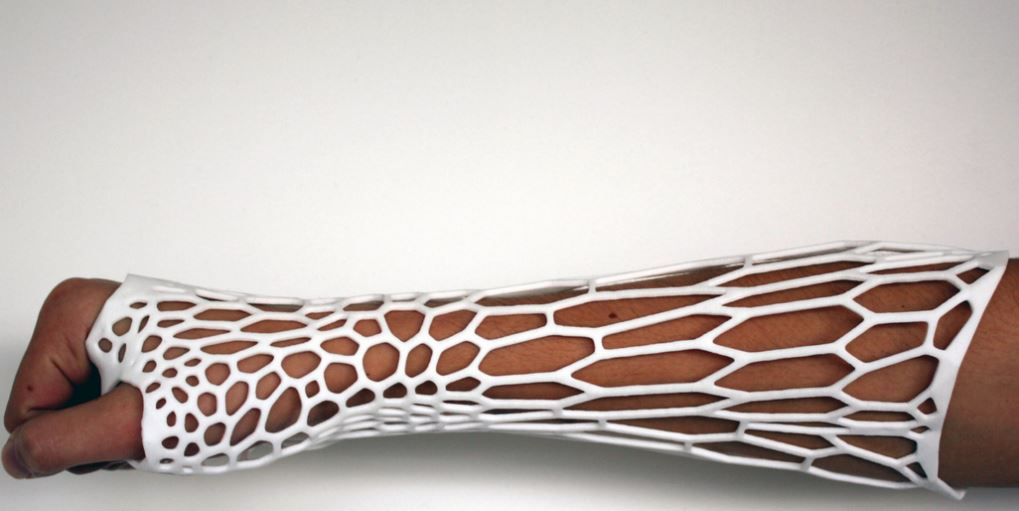
\includegraphics[width=\textwidth]{armPlaster}
  \end{minipage}
  \hfill
  \begin{minipage}[b]{0.45\textwidth}
    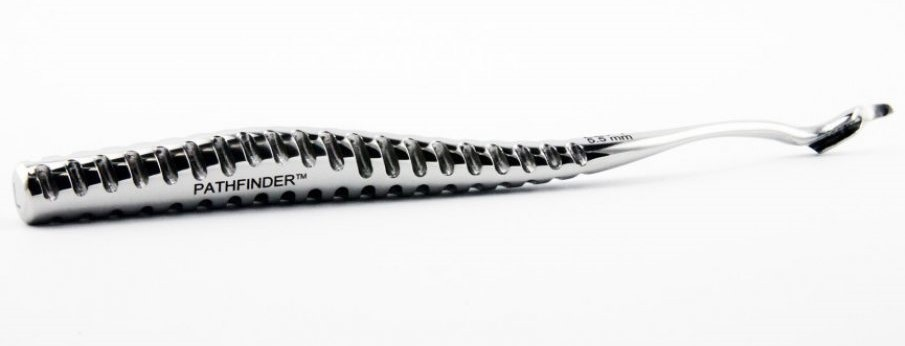
\includegraphics[width=\textwidth]{surgicalTool}
  \end{minipage}
  \\[5pt]
  \begin{minipage}[t]{0.45\textwidth}
    \caption{Arm plaster made with AM}
  \end{minipage}
  \hfill
  \begin{minipage}[t]{0.45\textwidth}
    \caption{specific surgical tool made using AM}
  \end{minipage}
\end{figure}
\subsection{Aviation industry}
Although AM is not primary production technology in aviation field, it can open great deal of possibilities. Many parts for aviation purposes are complexly shaped, and therefore complicated for machining. When a part from solid titanium block is machined to shape of i.e. turbine blade, it can mean that most of the material is machined away, even more than 80\%. Waste titanium can be recycled, but still the price of such titanium solid block is in range of thousands of EUR. When using PBF technology with titanium powder, we could eliminate the waste material, reducing the initial price of material. Still it is true that extra machining and polishing of such part would be required after, which could increase the costs, saved on material.
\subsection{Automotive industry}
Car production is, and probably will remain, thing of mass production. Yet, there is still place where AM can prove itself as useful. Before mass production, prototype making is again essential part, and therefore great deal of attention is always paid not to make mistakes during series preparation.\\
Lightweight metals such as aluminum can be utilized for functional parts such as valves, canals or tubes designed for specific car type. Polymers also can be used for interior design, i.e. during stage of preparing "non-stressed" parts such as handles, coverings or panel parts - here AM can be handy for visualizing the interior.
\subsection{Architecture or design}
The reasons of AM being useful in this field is probably apparent from previous description - designers more than others can appreciate shape-free manufacturing, and not having to bother with limitations of conventional manufacturing. 
\subsection{Educational purposes}
This field might be found not as significant as others. Still, the fact is teachers and lecturers at high schools or universities could easily make use of AM during lecturing. For example, teaching biology or chemistry often require lots of teaching supplies, such as model of skeleton or models of chemical compounds to visualize chemical bonds. These supplies are often expensive, because there are not that many schools buying such supplies. Result is low demand for such items, and higher price - body part models can cost hundreds of EUR. With AM, teachers could only download / create desired model such as human organ or chemical bond model and print it, all that for fraction of the original price.
%
%
%
\chapter{Materials for use in AM}
The scale of materials usable for purposes of AM is very wide. We can today print objects from different plastics like Nylon, polystyrene and others. Objects can be printed out of common metals such as steel and it's alloys, titanium, aluminum and others. Certain technologies make it possible to print even sand parts. Other methods enable building colorful parts. Since there are so many materials, we should be able to categorize them into logical groups. Materials used with each technology will be described in detail in related chapters – this is only brief summary of material options.\\
In following lines, some information might be slightly imprecise or misleading. The reason is, categorization of AM processes and related issues is very sophisticated and there are many slight differences among technologies. I will try to summarize some main ideas, but detailed description can be found in following chapters devoted to specific technologies.\\

\section{Material state}
One way of materials categorization is based on phase / physical state. Materials before printing process can be either solid or liquid. Solid materials can be used in forms of powder, wire or thin sheet / folia. Liquid materials are so far only photopolymers.
\subsection{Solid powder materials}
Powder materials are usually used for metal printing. Nevertheless, plastic and ceramic powders or sand might be used. Powder material can be processed by partially or fully melting and fusing together, creating a solid part with "Powder bed fusion" or "Directed energy deposition" technologies. Laser or electron beam is be used to melt the powder. Also, the powder can be glued by a special substance called binder – see "Binder jetting" technology. 
\subsection{Solid wire form materials}
Wire-form material is always used with "Fused deposition modeling" technology and rarely used with "Directed energy deposition". Within FDM, the plastic wire is partially melted and in controlled manner "spilled" and deposited. Due to its viscosity, one can precisely control the deposition process and it's precision. After solidification, plastic forms final object.
\subsection{Solid sheet form materials}
Sheet-form materials are used within the "Sheet lamination" technology. It uses thin sheet of metal, paper or basically any material, that can be cut and glued together. Each sheet equals one layer, that is cut into the shape of current cross-section.
\subsection{Liquid materials}
As mentioned, there are substances called photopolymers, used with AM. The principle is having a bath of photopolymer, which is precisely cured by light of specific wavelength. Where cured, material undergoes a chemical reaction, creating bonds between separate molecules and solidifying. "Stereolitography" of "Material jetting" commonly use photopolymers. In latter chapters, materials will be described more.\\
%
%
\section{Chemical composition}
We might also want to group materials based on their chemical composition. I will not fully describe chemical properties of materials like type of molecule bonds. Still, easily we can distinguish between main groups of materials.
\subsection{Metals}
Metals are generally materials that are good electricity conductors. This property is related to their other properties. Metals have generally higher yield strength (hundreds of MPa), very variable thermal expansion coefficient and medium-high melting point (important for heat curing of metals). They are usually also able to withstand some plastic deformation and do not absorp water.
\subsection{Plastic}
Other category is group of plastic materials. These materials have much lower yield strength, thus are not suitable for functional stressed parts. Usually they do not conduct electricity well and have low thermal conductivity coefficient, but higher heat expansion coefficient. Their melting / glass transition point is much lower than metal melting points, so they are easier to cure in this way.
\subsection{Ceramics}
Third category of materials used in AM are ceramic materials. Curing process is usually using ceramic powder. Melting point of ceramics is generally slightly higher than commonly used metals, but there can be exceptions. Ceramics is very hard and strong, yet brittle material. This property can be found problematic in AM. Because ceramics show almost no plastic behavior, they crack easily once they reach yield strength. This makes ceramics harder to process this way - during printing, rapid temperature gradients occur, causing thermal stresses and cracking.
\subsection{Photopolymers}
Among other materials are i.e. photopolymers. Even though they are plastic – polymers, I'd like to distinguish between them and other plastic materials, because they differ fundamentally in curing process. Default state of photopolymers is liquid, and it consists of more types of additives to make curing with light easier. Depending on point of view, they can therefore be considered different material from other plastics used in AM.
\subsection{Others}
Also, mixtures of different materials should be mentioned. Same we can make metal alloys of specific composition, we are able to incorporate small particles into plastic wires for FDM printing, like bronze of wood. If we have kind of material, consisting of 40\% wooden particles and 60\% polymer holding wooden  particles together, it is among one’s preference to say about which material are we talking about.\cite{WoodenFilament}
\section{Material processing}
Among other ways, we can also divide materials by the way of their processing.
\subsection{Heat processing} Some materials are processed by heat. They are fully or partially melted, and after cooling, material (like in most processes using metal powders) fuses or solidifies together into single physical object. Powerful lasers, or in case of conductive materials electron beam can be used instead as the heat source.
\subsection{Light processing}
On the other hand, liquid photopolymers are cured by light. Photons of specific wavelength (either UV, visible or other) initiate chemical reaction within material, causing creation of new chemical bonds and solidification.
\subsection{Other processing}
Binder jetting is the only technology, which basically doesn't process the material at all – it only binds the material together with special glue, called binder. The is no change happening of properties of the material, but the strength of the final part is limited by strength of binding particles by binder.\\
Also, with "Laminated object manufacturing" the sheets have to stick to themselves, which can be done using some special binding agent or glue.

\section{Common problems of material processing}
What we should realize when thinking about processing materials, are problems we are bringing along. Heat processes are related with thermal stresses, expansion / contraction and subsequent curling, warping and cracking. Similar issue is related to curing photopolymers, where curling and warping is caused not by heat, but by change of volume of material when changing state of matter. This is unique to binder jetting technology, which doesn't have to deal with these issues – as will be discussed in dedicated chapter.\\
It is not always necessary to strictly distinguish between different materials. Instead of having fixed table of categorized materials, we should have complex knowledge of different kinds, their properties, pros and cons. 

\chapter{Photopolymerization}
Photopolymerization technology, also called "Vat Photopolymerization" or "Stereolithography" (hereinafter abbreviated as SLA), was the first introduced AM technology on the market. It utilizes ultimately photopolymers as default materials. Photopolymers were developed in 60s, yet SLA appeared aprox. 20 years later. Since then, SLA machines has improved, along with available photopolymer materials.\\
SLA has many specifics of ongoing processes, resulting in both advantages and disadvantages of this technology. In this chapter, I will describe the general approach of this technology and relevant problematic, curing process itself, material properties and mention the overall conclusion of SLA.
\section{Stereolitography in general}
SLA is no exception in relation to patent problematic - patents used to determine the direction of SLA development. That is not true anymore, since 25 years validity of most of relevant patents has recently ended. As some company patented some SLA specific approach, other companies had to come up with different solution to the same technical problem. Same applies for all other technologies, that can be newer and patents might be still valid. SLA is therefore versatile technology with SLA machines varying in many parameters. Among those parameters are build speed, machine reliability, precision, price and many more.\\
The biggest difference among SLA machines is given by \textbf{different approaches} to curing individual layers, as seen in fig 4.1. For now, let's summarize what all SLA machines have in common.
\\SLA can also be called "Vat photopolymerization" because a vat is always present - a container, of which content is the prohopolymer resin. Typically, the volume of the container is in range of several liters up to more than cubic meter of the resin - the amount of material it can hold. Above the vat, there is the source of radiation, used to chemically process the resin. This system, utilizing optics and other devices, is located above the vat so that it can be directed on the resin surface and cure the top layer of the resin.\\
The source of the radiation is also one of the parameters of SLA machines. Typically, machines utilize \textbf{UV light}, sometimes visible light, both in form of a laser. Other sources of radiation, such as electron beam or gamma ray, might be used. It also depends on the processed material - the ultimate condition for the curing process is that material has to undergo chemical reaction to solidify. All of these radiation sources can be used to deliver energy to the resin, and initialize the reaction. Again, used lasers / other sources can vary in terms of their power, spot size, material requirements and such.

\begin{figure}[t]
  \centering
  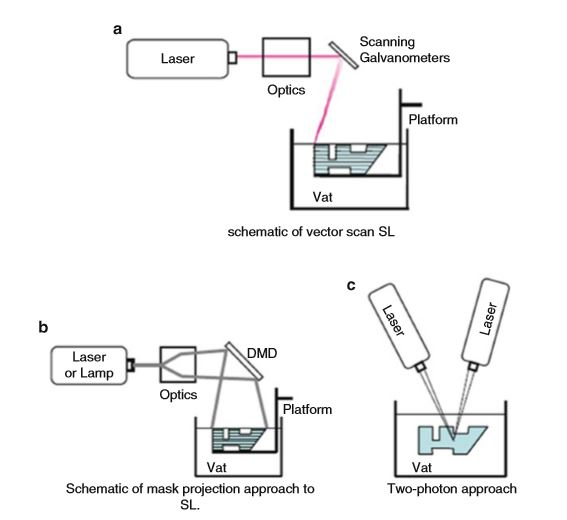
\includegraphics[width=0.8\textwidth]{SLAillustration}
  \caption{Illustration of SLA technologies}
\end{figure}
%
\section{Curing process} 
It was mentioned that there are more approaches within SLA of how to cure a layer of the resin - the easiest sorting criteria for types of SLA machines. With these approaches described in following section, fig. 4.1 is added for illustration.
\subsection{Spot scanning}
The first approach is the most common one - layer is cured by a laser, which is projected onto the resin surface by mirrors. Laser is focused in very small area, thus called \textbf{spot scanning} or \textbf{point scanning}. By changing the angle of the mirrors, we can control and move the location of laser spot on the resin surface. By constantly changing the mirror angles, we create a path - trajectory of the laser. When a laser moves past a point on the resin surface, it leaves solidified material behind - where the laser points, the material becomes solid. This approach is the oldest one and most of SLA machines utilize this approach. Similar approach is used with Powder Bed Fusion, where laser or electron beam is used to scan the surface of powder layer, causing solidification by melting particles together.
\subsection{Mask projection with DMD}
Another approach utilize Digital micromirror devices - DMD to cure single layer at once. With spot scanning, curing a layer can take a lot of time, because the laser has to scan the whole cross-section surface, meaning the path the laser has to scan is very long. If we use DMD, we can speed up the process significantly. That is, because with mask-projection technology, we \textbf{irradiate single layer simultaneously}.\\
DMD is basically a 2D array of microscopic mirrors, that can be controlled and positioned individually. These DMD chips can have, for example, resolution of 1024x768 pixels, where each pixel represents a single micromirror. This micromirror can be switch between "on/off" state, so we can set a shape, that will reflect light, while remaining pixels will not reflect the light. Strictly speaking, we change the angle of the mirror between two positions, we don't turn the mirror off. When the light is projected onto the micromirror, we can control individual pixels - mirrors to control the shape, reflected onto cured layer. The light projected onto DMD, of course, has to be the kind of light photopolymer is sensitive to.\\
With mask projection SLA process, we start by spreading a layer of photopolymer resin. Then, we set the DMD to reflect the shape of first layer, and then project light onto the surface, reflecting from DMD. After curing a layer, light source is turned off and next layer of resin is applied on the top of previous layer. Then, we set the shape of DMD to reflect the second layer and irradiate it. Repeating this process, we get a final part.\\
%
\begin{wrapfigure}{r}{0.35\textwidth}
 	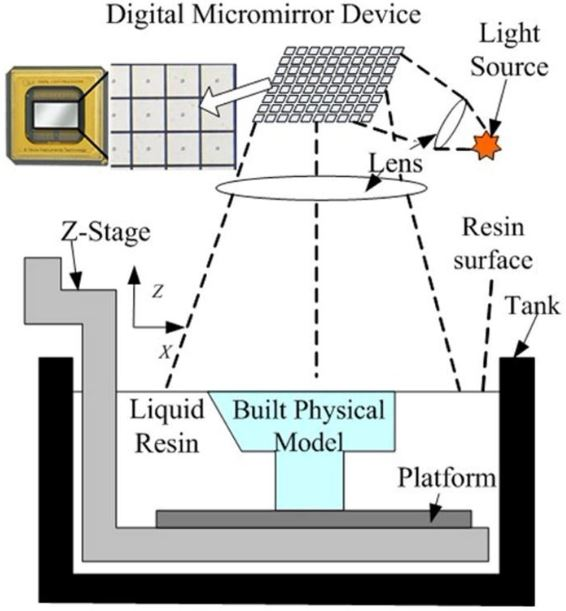
\includegraphics[width=0.35\textwidth, angle=180]{DMD}
	\caption{Utilizing Digital micromirror with SLA}
\end{wrapfigure}
%
The \textbf{speed} of mask projection is the \textbf{biggest advantage}. The general process of SLA can be sped up more than 10x compared to spot scanning. On the contrary, the limiting factor of DMD approach is the individual micromirrors size. Let's say we reflect the light from DMD to the surface of 20x20cm. If DMD has resolution of 1000x1000 pixels, then 1 pixel has resolution of 0.2mm, or 200 microns. Such resolution would very low and insufficient. In order to increase the resolution, we would have to either increase the resolution of DMD, or decrease the surface light is reflected to - make build area smaller. Higher resolution DMD can be costly and usually the resolution is lower than 3000 pixels on the longer side. The other solution, making build area smaller, is a obvious limitation itself.\\
For the information to be complete, it should be noted that DMD is not the only device enabling shape projection onto the resin. Apart from DMDs, LCD display or spatial light modulator can be used. DMD is here used as an example for mask-projection approach.\\
%
\subsection{Two photon approach}
Third approach is very different from previous spot scanning / mask projection. It was developed for manufacturing \textbf{very small and precise parts}. Today, parts smaller than 1 $\mu$m have been produced. More standard size of produced parts is in range of few up to tens of $\mu$m.\\
The basic principle is, we have a small container of resin, and we direct two separate lasers inside the container. One laser is not enough powerful to cause the chemical reaction and solidification. This occurs only where the beams of lasers intersect. Only in this very small region, that can be in ranges smaller than 100nm, the energy density is high enough to cure the resin. Due to this fact, the precision of built part can be greatly increased compared to other SLA approaches, at the expense of build speed. Also, there is no need for re-coating, since the process happens inside of the container, not on the surface, being another advantage of two-photon approach. The viscosity of the resin is usually high enough to prevent the part from flowing away before it is fully cured.
%
\begin{figure}[h]
\centering
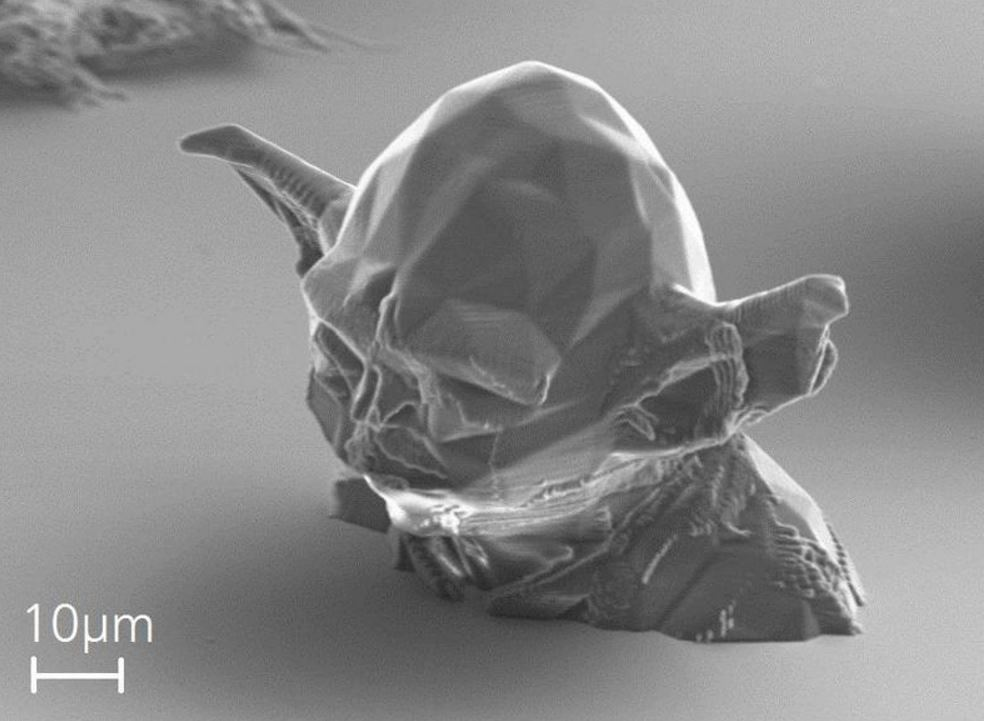
\includegraphics[scale=0.5]{yoda}
\caption{Image of a small statue of popular figure of YODA, made with two-photon SLA}
\end{figure}
%
\section{Photopolymer materials}
In this section, the \cite{AMT} is referring to \cite{SLAmaterials} as to primary source of following information on photopolymer materials.\\
\\
Different radiation sources used for resin curing were mentioned. From all of them, only light from visible or ultraviolet spectra is utilized within commercial AM machines; others remain in the field of research.\\
As SLA uses polymers, they divide into categories of thermoplastic and \textbf{thermoset} polymers. For their properties only thermoplastic polymers are used. Thermoset polymers are unsuitable for SLA, since they can't re-melt.\\
When we focus on thermoplastic polymers, we can put together list of material properties which determines how suitable the material is for SLA processing. Among others, we are often interested in reactivity / sensitivity to radiation, mechanical properties of the cured material (strength, brittleness) and amount of shrinkage due to phase transformation. The shrinkage is caused  by polymer molecules being smaller than  size of all previous uncured monomer molecules.\\
Epoxy resins are used today. Before that, acrylate compounds were utilized. These two material categories have very different properties - acrylates tend to shrink more and are therefore difficult to process, but epoxy resins have slow reaction (photo) speed and are more brittle. Accordingly, often a mixture of these two groups is used to achieve desired properties of the final part.\\
Among ingredients such as the epoxy resin / acrylate itself, the material mixture for SLA consists of more ingredients, which affect it's other properties. Namely, "photoinitiator, reactive diluents, flixibilizers and liquid monomers" \cite[p. ~67]{AMT} are usually present, where each constituent has a certain role. For instance, photoinitiator component works as a catalyst, helping to start the chain reaction and cross-linking of monomer molecules.
%
%
%
\section{Curing of materials}
%
\subsection{Theory and math of curing}
When talking about curing the resin to solidify, we have to consider the time factor - all individual processes during build take time. Same applies for curing - due to limited power of laser, speed of chemical reaction and other factors that can't be overlooked. In other words, we can't speed up the build process as we want, because curing processes themselves always take some time.\\
When calculating basic build parameters, the most important parameter is the amount of laser energy, absorbed by the resin. There is critical amount of energy, which resin needs to absorb in order to undergo the chemical reaction. This parameter or energy per amount of material [$J/kg$] vary. With SLA, because of using finite layer thickness, this parameter is usually replaced by critical exposure with units of [$mJ/mm^2$], meaning critical amount of laser energy absorbed by 1mm$^2$.\\
So we have to account for parameter of laser properties. Even though laser is focused into very small area, the energy density of laser vary in this area - in the center of laser spot will be different energy density and exposure, compared to the edge of the laser spot.\\
Following parameter, that also has to be remembered, is penetration of the laser. When the light hits the surface, part of the light will be absorbed in the form of energy, and the rest of the light will penetrate deeper into the resin. This results in different energy density and exposure, depending on depth under the surface. There is parameter called critical depth. Above this depth, for a given laser set-up exposure of the resin is high enough for the reaction to happen. Below this depth, laser light is too scattered and the energy density is below critical and no solidification will occur.\\
All given parameters combined give us an equation, where the exposure of material if function of all spacial coordinates. According this function of exposure, we can border the region, where exposure is greater than critical exposure - the area where chemical reaction will occur. Outside of this region, the raw material will remain liquid, for the exposure was not sufficient. Because energy = power x time, with given laser power, there is minimal time the laser has to irradiate a certain place. Given laser power, we can calculate maximal build speed. From further mathematical equations used for description of ongoing SLA processes, it can be derived that a cross-section shape of cured line is a \textbf{parabola}.\\
%
\subsection{Scan patterns and other issues}
%
\begin{figure}[!t]
  \centering
  \begin{minipage}[b]{0.45\textwidth}
    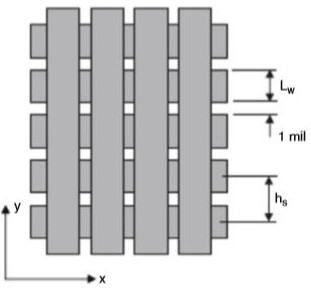
\includegraphics[width=\textwidth]{weave1}
  \end{minipage}
  \hfill
  \begin{minipage}[b]{0.45\textwidth}
    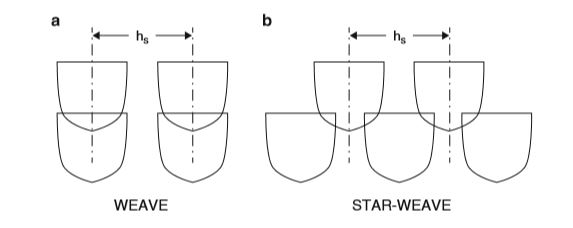
\includegraphics[width=\textwidth]{weave2}
  \end{minipage}
  \\[1pt]
  \begin{minipage}[t]{0.45\textwidth}
    \caption{Original WEAVE pattern}
  \end{minipage}
  \hfill
  \begin{minipage}[t]{0.45\textwidth}
    \caption{Comparison or WEAVE / STAR WEAVE patterns}
  \end{minipage}
  \\[10pt]
  \begin{minipage}[t]{\textwidth}
  \centering
  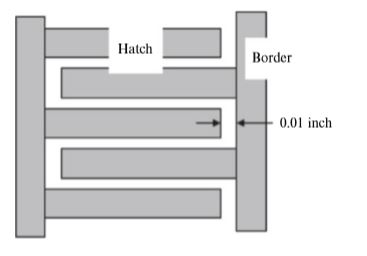
\includegraphics[scale=0.8]{retractedWeave}
  \caption{Retracted WEAVE scan pattern with improved shrinkage endurance}
  \end{minipage}
  \\[20pt]
\end{figure}
%
Even if we are able to precisely describe the curing process, it is not enough to secure a successful build. The curing process is happening on a small scale, but the overall build process brings other problems. For example, with describing curing process, we haven't accounted yet for shrinkage and residual stresses, anisotropic behavior caused by laser scanning trajectory, overlapping of cured lines, or layers sticking to previous / following layers.\\
Problem of overlapping layers is, that we have to irradiate more energy to the resin than the critical exposure. Reason being, the current layer has to cure into previous layer. This re-curing of previously cured layer requires some additional energy, by which critical exposure has to be increased, decreasing theoretical maximum build speed.\\
Problem of shrinkage and anisotropy of the build is interrelated. Simple explanation can be given by following example: We are curing a single cross section of full square. Let's say we cure the circumference of the shape first. Than, we have to cure the infill - inside of the circumference. One of the options is to cure horizontal or vertical lines, parallel to one of square borders. If we go from upper border to bottom border, than immediately after curing first upper infill lines, the upper part of square will tend to shrink. This will cause either decreasing dimension of the square, or internal stresses which will remain be present.  By this simple approach, we are causing anisotropy, since we have a scanning pattern preferring a single line direction. This issue we can try to eliminate by curing next layer perpendicular to previous one. By switching the pattern, to some extent, we eliminate the anisotropic property of the build - the build as a whole is more or less isotropical, but individual layers vary from each other. Also, we should bear in mind, that if the part shrinkage is problem not only for causing stresses, but also for changing dimensons of the part. The resolution of SLA printer can be in range of tens of microns, so even if the shrinkage will not ruin the build, we might not be able to stick to our desired part dimension - the real part built might be smaller due to shrinkage.\\
Next issue to deal with is overlapping of parallel cured lines. Obviously, two adjacent lines also have to be cured together for better structural integrity of the part. On the contrary, this overlapping also causes deflection of already cured sections, and adds another source of anisotropy to the build.
To account for all of mentioned and other related issues, certain scanning patterns for SLA were developed. Here, with scanning pattern is meant how the infill of layer circumference is cured. These scan patterns are called WEAVE and STAR-WEAVE. Further improved comes the retracted hatch WEAVE scan pattern. Illustration of these patterns are in fig. 4.5 , 4.6 and 4.7. With these scan patterns, negative effects of SLA builds can be minimized for securing successful build.

%
\section{Conclusion}
All necessary being said, let's summarize the pros and cons of SLA technology.
%
\begin{itemize}
\pro \textbf{Part precision}\\
Not only with two-photon approach, we can achieve parts of high precision, to which only some other technologies are comparable.
\pro \textbf{Surface finish}\\
Surface roughness is incomparably better than of parts made with i.e. DED or FDM technologies.
\pro \textbf{Build speed}\\
Although build speed is a relative term and depends on build set-up and parameters, SLA is often quicker than other technologies.
\\[10pt]
\con \textbf{Support structures}\\
Need for support structures is present with SLA. When machine operator removes the built part, it requires cleaning from the resin, and often mechanical removal of the support structures.
\con \textbf{Materials}\\
As the term photopolymerization implies, range of available materials is limited to thermoplastic polymers.
\con \textbf{Price}\\
Furthermore, same as SLA machines themselves, these materials are often very expensive. Single liter of the resin can cost hundreds of EUR. With biggest nowadays SLA machine, even filling the container full can cost thousands of EUR. The price of big machines, able to print more than 2 meters wide objects, can be higher than 500 000 EUR.
\end{itemize}

\chapter{Powder Bed Fusion}
Basic description
Materials used
Mechanisms, differences - chemical, melting, sls, 4th / heat source / 
Challenges, problems
Pros / cons

Powder bed fusion ("PBF") is a technology, that is very versatile compared to other AM technologies. It is able to utilize variety of materials and final products are often fully dense functional parts. The trade-off for it's abilities is in the need to understand all simultaneous processes during PBF printing, and need to set all print parameters carefully. Also, post-processing of the part is required, unit for recycling the powder is almost necessary and materials themselves are expensive. Therefore, even though PBF is superior to other AM technologies and in some ways even to CNC machining, it is very expensive to operate and handle.

\section{Basic operation principles}
As follows from the name, PBF uses material in a form of powder. Although very simplifying, we can say that any material in form of small particles that can be melted together can be utilized. We can use metals, polymers, ceramics and composites, but i.e. machines using polymers and machines using metals face often very different problems. Therefore we have to bear in mind, that even among PBF machines, there are big differences and a single machine is usually not capable of processing any material, but rather only polymers / metals and so.
\\
\todo{Obrazek sestavy}
In the picture, we see a typical PBF machine setup. The powder is held in a heated container. The build platform is the place where the actual part is built. When a current layer is cured, the build platform is lowered by one layer thickness, and new layer is moved from the powder container and spread onto the build platform by specific spreading mechanism. The newly spread powder has to be uniform, precisely leveled and packed.

\section{Classification of Powder Bed Fusion processes}
Hello
\section{Materials for Powder Bed Fusion}
Hello


\chapter*{Tensile strength of parts printed with FDM}
The technology of Fused Deposition Modeling, or Fused Filament Fabrication (FDM/FFF) was described previously. This thesis consists also of practical and experimental section, which is based on FDM. The task was to find, what effect do \textbf{print parameters of FDM}, such as layer thickness, infill amount etc, have on \textbf{strength} of the final part.\\
There are multiple reasons why such knowledge is valuable and important. Obvious reasons are, during parts design we always have to be aware of the part production process - different manufacturing procedures may result in different properties of the same part geometry. This is mostly due to anisotropical nature of such processes. When we are talking about FDM, the process is very anisotropical with parts having different properties in X/Z build direction (plane of single layer) and Z direction (vertical direction of build). Probably all kinds of macroscopic properties will show some amount of anisotropy, such as heat conductivity or electric conductivity. This is generally applicable on AM, i.e. plastics used with FDM are bad electricity conductors. For mechanical engineering, however, the crucial property that will vary with changing direction is strength and elongation of the material.\\
Another important reason for such research is that we should be able to make a direct comparison between strength of part of the same geometry and made of the same material, but produced using different technologies. Particularly useful is the ability to compare parts made with \textbf{injection molding} and \textbf{additive manufacturing}. Both are using polymer materials and processing them by heat. For injection molding, the part will also be somewhat anisotropical, which is caused by the flow direction of the plastic. Compared to FDM however, injection molded parts will be much more isotropical and uniform.\\
The difference here can be of great significance, when we are considering production of functional, i.e. stressed parts. We know that injection molding and AM are on the opposite ends of the spectra of production rate, with molding being extremely productive with high quantities and AM being very slow. Nonetheless, if we find out that only very limited of parts is to made made (ranges of $10^0$ up to $10^3$ pieces), it is rational to think of AM instead of injection molding. On the contrary, AM produced parts due to it's nature will show different strength and elongation. Therefore production technology has to be accounted for before the production itself.
\todo[inline]{misto pro nejakz obrazek}
\newpage
Following parameters were to be examined:
\begin{itemize}
\item Layer thickness\\
	Different thickness of individual layers, range from 0.1 - 0.25 mm
\item Infill\\
	Amount of infill, range from hollow = 0\% up to full = 100\%
\item Print temperature\\
	Different setting of the constant nozzle temperature during extrusion
\item Infill raster orientation\\
	Orientation of rectilinear raster pattern, angle with edges 0° - 45°
\item Layer orientation\\
	Part build on different sides - different orientation of build
\\[10pt]
\item \textbf{Default parameters}\\
Layer thickness 0.1mm\\
Infill 100\%, rectilinear pattern\\
Print temperature 240°C\\
Infill raster orientation 45°\\
Layer orientation - parallel to stress direction
\end{itemize}

Other print settings and parameters remained constant, and are listed as follows:\\
\begin{itemize}
\item Material\\
	PETG
\item Nozzle diameter\\
	1.75mm/0.4mm
\item Overlap of material\\
	25\%
\item Number of shell lines\\
	3 outside shell lines (inside is infill pattern)
\item Number of top layers\\
	???
\item Bottom layers\\
	???
\item Other\\
	IDK
\end{itemize}
For making test specimen, 3D printer Prusa I3, borrowed from Prusa company (mentioned in acknowledgements) was used. Slicer software used for Gcode generation was Prusa slicer ver. 1.31.6. The test specimen has a shape as in fig. ??? \todo{obrazek okotovany test specimen}. The shape is given by the ASTM D638 standard, used for plastic parts made by injection molding or machining. Up to this date there is no other generally accepted standard for 3D printing specimen for tensile strength testing. 
\todo[inline]{jaka tiskarna, vypsat vsechny parametry, jaky software, material\\
popsat trhani, ceh jsme si vsimli, jake vzorky vyhodit jake ne\\
jaka norma astm d638, test specimen tvar\\
vliv rychlosti deformace, rychlost dle normy}

\tableofcontents
\listoftodos

\begin{thebibliography}{99}
	\bibitem{AMT}
	GIBSON, I. \& ROSEN, D. \& STUCKER, B.,
	2015.
	Additive manufacturing technologies
	2nd ed.
	Springer:
	New York, Heidelberg, Dordrecht
	ISBN 978-1-4939-2112-6
	
	\bibitem{FirstPatent}
	Hull, Charles W.
	Apparatus for production of three-dimensional objects by stereolithography,
	US4575330 A,
	USA,
	8.8.1984
	
	\bibitem{JointReplacement}
	Trebše, R.
	Infected Total Joint Atrhoplasty - The algorithmic Approach,
	2012,
	ISBN: 978-1-4471-2481-8
	
	\bibitem{DentalPrinter}
	ENVISIONTEC,
	[online],
	last revision 13.3.2017,
	<https://envisiontec.com/3d-printers/desktop-3d-printers/vida>
	
	\bibitem{AMOrigins}
	3D PRINTING INDUSTRY,
	[online],
	2017,
	last revision 13.3.2017,
	<https://3dprintingindustry.com/3d-printing-basics-free-beginners-guide/history/>
	
	\bibitem{WoodenFilament}
	MATTER HACKERS,
	[online],
	2017,
	last revision 13.3.2017,
	<https://www.matterhackers.com/store/3d-printer-filament/175mm-wood-filament-light-cherry-0.25-kg>
	
	\bibitem{SLAmaterials}
	Jacobs PF (1992)
	Rapid prototyping \& manufacturing,
	fundamentals of stereolitography,
	SME,
	New York
	
\end{thebibliography}

\end{document}
